\section{Background}

In this section I'll provide a self-contained explanation of Yao's Garbled Circuits.

Multi-party computation, or MPC, is a kind of cryptographic protocol where several people send some messages back and forth. The point of an MPC protocol is to compute the output of some function on private inputs held by each party, but without those parties needing to share their inputs. If you could trust someone to do the computation and keep everyone's inputs secret, then the calculation would be easy. MPC removes the need to trust other parties.

Multi-party computation can refer to any kind of computation involving any number of parties (greater than one). In this paper, I focus on one protocol under this umbrella, Yao's Garbled Circuits, which performs computations between two parties by evaluating a Boolean circuit.

\subsection{Boolean Circuits}

\begin{figure}[b]
	\centering
	\begin{tikzpicture}
		\node[and port] (andA) at (0, 0){};
		\node[xor port] (xor)  at (3, .7){};
		\node[and port] (andB) at (3,-.7){};
		\draw (xor.in 1)  -- ++(-5, 0)
		      (andB.in 2) -- ++(-5, 0)
		      (andA.in 1) -| ++(-1, .7) node [below right] {A}
		      (andA.in 2) -| ++(-1,-.7) node [above right] {B}
		      (xor.in 2)  -| (andA.out) node [      right] {C}
		      (andB.in 1) -| (andA.out)
		      (xor.out)  node [above] {D} -- ++(1, 0)
		      (andB.out) node [above] {E} -- ++(1, 0);
	\end{tikzpicture}
	\caption{An example Boolean circuit with one XOR gate and two AND gates. The inputs wires are on the left columns and the outputs are on the right column.}%
	\label{fig:circuit}
\end{figure}

A Boolean circuit is a collection of logic gates connected together by wires. Each wire receives a label, with the computation's inputs assigned to the wires on the left. Each gate then compares the labels on its inputs to the gate's own lookup table to determine what label to assign to its output wire on the right. The contents of the lookup table determine how the gate behaves, and we give names to several common sets of table contents. For example, if 0 and 1 are the possible labels for each wire, and correspond to False and True respectively, then Tab.~\ref{tab:truth-table} shows an AND gate, an XOR gate, and another AND gate, left-to-right.

Circuits like these can compute any mathematical expression. (For usage in MPC, circuits can't have loops, so any looping algorithm will need its loops unrolled first.)

\begin{table}[ht]
	\centering % empty columns are easier than whatever is proper
	\begin{tabular}{cc|c   cc   cc|c   cc   cc|c}
		A & B & C   &&&   A & C & D   &&&   C & B & E \\
		\cmidrule{1-3}    \cmidrule{6-8}    \cmidrule{11-13}
		0 & 0 & 0   &&&   0 & 0 & 0   &&&   0 & 0 & 0 \\
		0 & 1 & 0   &&&   0 & 1 & 1   &&&   0 & 1 & 0 \\
		1 & 0 & 0   &&&   1 & 0 & 1   &&&   1 & 0 & 0 \\
		1 & 1 & 1   &&&   1 & 1 & 0   &&&   1 & 1 & 1 \\
	\end{tabular}
	\caption{Truth tables for the gates in Fig.~\ref{fig:circuit}. Each column is labeled to match a wire and each row matches an input combination to an output value.}%
	\label{tab:truth-table}
\end{table}

To perform a computation with a circuit, you need to evaluate it. First, assign input labels to the wires on the left. Then, for each gate with all inputs labeled, check its truth table to determine which label to give the output wire. Note that gates are referred to by their output wire. Continue until all of the output wires are labeled, and then interpret those final labels for the result. For example, if every wire is labeled either 0 or 1, then the input to the circuit can be determined by applying the binary representation of a number, one bit at a time, to each wire. Similarly, the output labels can be concatenated as bits of the output number.

The Boolean circuit shown in Fig.~\ref{fig:circuit} is too small to have much practical use. For comparison, even simple math operations like multiplication and square roots can require tens or hundreds of thousands of gates\cite{bristol}.

\subsection{Oblivious Transfers}
An oblivious transfer is a cryptographic primitive used in garbled circuits. It allows Bob to make a choice about which item to receive from Alice, without Alice knowing which item Bob chose, and without Bob learning anything about the item he didn't choose\cite{FirstOT}.

You can picture this as Bob sending Alice two empty boxes, labeled 0 and 1, shown in Fig.~\ref{fig:OT}. Alice puts messages in each box, locks them, and sends them back, but Bob only made the key to box 1, a choice he made up-front before sending anything to Alice. Alice doesn't know which message Bob got, since the locks on the boxes look the same to her. Bob doesn't learn anything about the other message since the cryptography involved prevents the possibility of Bob creating two functional keys.

\begin{figure}[ht]
	\centering
	\begin{tikzpicture}[ scale=.8,
			IOarrow/.style={->, >=stealth, line width=.5mm},
			flowarrow/.style={->, >=stealth, line width=1mm, auto}
		]
		\draw[dashed] (0,-5) -- (0,5);

		\draw (-4,5) node [below] {\large{Bob}};
		\draw (4,5)  node [below] {\large{Alice}};
		
		\lockshape{-5,2}{0} % step 1
		\lockshape{-3,2}{1}
		% 1 -> 2 arrow
		\draw[flowarrow, bend right=20] (-1,1.5) -- (1,1);

		\lockshape{5,-1}{1} % step 2
		\draw (5,.5) node [above] (txt) {``$\psi$''};
		\draw[IOarrow] (txt) -- (lastBox);
		\lockshape{3,-1}{0}
		\draw (3,.5) node [above] (txt) {``$\pi$''};
		\draw[IOarrow] (txt) -- (lastBox);
		\littlekey{-3,3.2}{1}

		% horizontal divider
		\draw[dashed] (-6.5,0) -- (0,0) (6.5,0);
		% 2 -> 3 arrow
		\draw[flowarrow, bend right=20] (1,-1) -- (-1,-1.5);

		\lockshape{-5,-2.5}{0} % step 3
		\draw (-5,-4) node [below] (txt) {???};
		\draw[IOarrow] (lastBox) -- (txt);
		\lockshape{-3,-2.5}{1}
		\draw (-3,-4) node [below] (txt) {``$\psi$''};
		\draw[IOarrow] (lastBox) -- (txt);
		\littlekey{-3,-1.3}{1}

	\end{tikzpicture}
	\caption{The oblivious transfer, shown with locks and boxes. Bob sends alice two empty boxes, one of which he has already decided he will be unable to open. Alice places different items into each, and sends them back to Bob. Bob opens the box he selected earlier. Alice does not know which item Bob received, and Bob knows nothing about the item he didn't receive.}%
	\label{fig:OT}
\end{figure}

%The process is similar to that of the Diffie-Hellman key exchange used when initiating an HTTPS connection (and many other secure protocols)\cite{FirstOT}. Alice generates and sends Bob a public key, then encrypts and sends two random messages (preparation material for Bob's boxes). Bob then chooses one of these messages and combines it with an encrypted random value of his own and sends it back to Alice. Alice receives Bob's encrypted choice (essentially two boxes combined into one value) and removes her own random value from before (opening the box),
\comment{this really needs more work. Or do I just direct the reader to Wikipedia?}

\subsection{Garbled Circuits}\label{sec:gc}
Boolean operations are represented by tables, but these tables don't have to map Trues and Falses, and in fact the outputs don't have to match the inputs at all. For example, in Fig.~\ref{fig:circuit} and Tab.~\ref{tab:truth-table}, wire A could instead have labels of $\psi$ and $\pi$ while wire B has labels of $\phi$ and $\delta$. Then gate C (the AND gate on the left) would then have a truth table that dictates the output label when the inputs are $\pi$ and $\delta$ or any other combination. Naturally, one can still evaluate a circuit without knowing which arbitrary labels correspond to True. This forms the basis for garbling.

The goal for Yao's Garbled Circuits is to allow one party to perform some transformation on a Boolean circuit such that the other party can evaluate the circuit blindly. If the garbler, traditionally named Alice, were to evaluate the circuit, she would know how the inputs correspond to Trues and Falses, and she is therefore ineligible to evaluate the circuit if the two parties wish to keep their inputs secret. If the evaluator, traditionally named Bob, could determine how the arbitrary labels correspond to True and False values, preserving privacy would be similarly impossible. Instead, we must find a way to completely obscure the function of a gate while still allowing Bob to evaluate it.

\begin{table}[t]
	\centering
	\begin{tabular}{cc|c   cc   cc|c   cc   cc|c}
		A & B & C &&& A      & B        & C                 &&& A     & B      & C \\
		\cmidrule{1-3}\cmidrule{6-8}                            \cmidrule{11-13}
		0 & 0 & 0 &&& $\psi$ & $\phi  $ & $\cap$            &&& $\psi$ & $\delta$ & $\cap$ \\
		0 & 1 & 0 &&& $\psi$ & $\delta$ & $\cap$            &&& $\pi $ & $\delta$ & $\Leftrightarrow$ \\
		1 & 0 & 0 &&& $\pi $ & $\phi  $ & $\cap$            &&& $\pi $ & $\phi$   & $\cap$ \\
		1 & 1 & 1 &&& $\pi $ & $\delta$ & $\Leftrightarrow$ &&& $\psi$ & $\phi$   & $\cap$ \\
	\end{tabular}
	\caption{The original truth table from Tab.~\ref{tab:truth-table} on the left and partially garbled in the center, and randomly permuted on the right. Each wire's labels have been substituted with an arbitrary pair that correspond to True and False. Note that even in the table on the right, it's possible to determine which arbitrary labels correspond to True versus False.}%
	\label{tab:garbled-table}
\end{table}

Naturally, seeing the truth table would reveal how the arbitrary labels correspond to True and False. Especially since Bob must know the whole circuit definition (for reasons that will become obvious in the next section), he will already know that gate C is an AND gate, and if he received the partially-garbled truth table shown in the center of Tab.~\ref{tab:garbled-table}, then he would immediately know that $\pi$, $\delta$, and $\Leftrightarrow$ all correspond to True because of the last row. Even without preserving the order, as shown in the table on the right, the asymmetry of the AND gate still gives away the values hidden under the arbitrary labels. Bob can look at the entire table and count that there are three instances of $\cap$ in the output and only one $\Leftrightarrow$, and conclude that $\Leftrightarrow$ must mean True.

The solution is for Alice to encrypt the output of each individual row of the randomly-permuted and arbitrarily-labeled table, using that row's inputs as keys. Then when Bob wishes to evaluate the circuit beginning with the labels on the left, he combines them to form a key with which he can unlock the correct output for each gate. The rest of the evaluation process proceeds as normal, but each gate evaluation now involves decryption. This way, Bob cannot observe the whole gate truth table like before, and therefore has no clues about the hidden meaning of the arbitrary labels.

At this point, it is easier to proceed with a different metaphor. Consider, instead of truth tables, a collection of four locked boxes, each with two key holes. Here, wire labels become keys such that each wire gets a unique pair of keys where one secretly corresponds to True and one to False. Then to evaluate a gate, you take the two inputs keys (wire labels) and open the only box that they fit in (decrypt the row of the truth table) to reveal the contents of the box, which is another key (the output column of the truth table which contains another wire label).

The process of evaluating the circuit is then Bob unlocking any box he has both keys for, and adding whatever key is inside to his collection as he goes. To begin the process, Alice prepares by making many random pairs of keys and locking them in boxes, and then sends these boxes to Bob. Once Bob has all of the keys that correspond to the inputs to the circuit, he can start unlocking boxes. When he does this, Bob is executing the circuit blindly without learning anything about the values in his computation. The whole garbled circuit is like an opaque machine that Bob drops his keys into, and then he ``turns the crank'' until the output comes out the other side.

Alice made all the boxes, so she can place the plaintext circuit outputs (0 and 1) in each final box on the right side of the circuit rather than a random key. It's her knowledge of the garbling transformation that's required to convert the answer from random keys and boxes to the result of the calculation.

Careful readers will have noticed a problem, though. How can Bob get the keys that correspond to Alice's inputs and his own inputs to begin the evaluation? Alice can simply send the keys that correspond to her input directly to Bob, since he doesn't know how they correspond to True and False values. For Bob's input, the solution is to use an oblivious transfer as described in the previous section.

Alice generates the true and false keys for every input bit. She can just give Bob the right key for her own input, since Bob doesn't know what it means, but she can't give Bob both keys for each of his inputs or he would be able to speculatively execute the circuit and he might be able to figure out her input. Bob also can't just ask for the key that corresponds to his input, because then Alice would know his input trivially. Instead, Bob requests the keys for each bit of his input with an oblivious transfer and Alice therefore does not know which keys he's receiving. Bob also does not receive any extra keys that would allow him to snoop on other possible circuit evaluation outcomes.

\begin{figure}[ht]
	\centering
	\begin{tikzpicture}[
		clearbox/.style={rectangle, draw, thick, minimum size=10mm},
		clearIO/.style={rectangle, thick, minimum size=10mm},
		garbledbox/.style={rectangle, draw, thick, minimum size=15mm,align=center},
		garbledIO/.style={rectangle, thick, minimum size=15mm, align=center},
		->,  % makes the edges directed
		>=stealth, % makes the arrow heads bold
		line width=.5mm,
		node distance=2cm,
		]
		\node[clearIO] (i)  {Input};
		\node[clearbox, right=of i,black!20!white] (c) {Circuit};
		\node[clearIO, right=of c] (o) {Output};
		\draw[dashed, black!10!white] (i) -- (c);
		\draw[dashed, black!10!white] (c) -- (o);
		
		\node[garbledbox, below=of c] (gc) {Garbled \\ Circuit};
		
		\node at ($(c)+(0,-1.33cm)$) [
			top color=black!20!white,
			bottom color=red,
			single arrow,
			minimum height=2cm,
			minimum width=10mm,
			inner sep=0mm,
			single arrow head extend=.1mm,
			rotate=270, single arrow
		] {};

		\node[garbledIO, below=of i] (gi) {Garbled \\ Input};
		\draw[red] (i)  -- (gi);
		\draw[blue] (gi) -- (gc);
		\node[garbledIO, below=of o] (go) {Garbled \\ Output};
		\draw[blue] (gc) -- (go);
		\draw[red] (go) -- (o);
	\end{tikzpicture}
	\caption{Circuit garbling as a translation. The red arrows show Alice's role and the blue arrows show Bob's. The greyed-out portion shows how a non-garbled circuit would be evaluated.}%
	\label{fig:garbling}
\end{figure}

The vertical arrows in Fig.~\ref{fig:garbling} are transformations to and from the garbled execution space that Bob works in. The horizontal arrows are computations within this garbled execution space. Since Alice knows about the transformation, she can't be the one to do the execution. Since Bob has all the inputs, he can't learn anything about the transformation. Together, though, they can perform the computation without either of them learning anything about the computation, including each other's inputs, except the final result.

\subsection{Yao's Garbled Circuits}
This protocol was first described by Andrew Yao in 1986 at that year's IEEE Annual Symposium on Foundations in Computer Science\cite{YaoGC}. In the most basic terms, one party ``garbles'' the circuit by encrypting and transposing the inputs to each logic gate, then sends the stream of garbled gates to a second party, who evaluates the garbled circuit with their own private inputs while learning nothing about the garbler's inputs.

Alice, who garbles the circuit, must get this new representation to Bob. If we assume they both already have the same circuit to begin with, and they agree on a way to sort the gates into a series, then Alice can send the new truth tables that she generated in that order. Further, since the truth tables are permuted randomly anyway, there's no need to send the input columns. This means that Alice only needs to send the encrypted outputs of each gate for each input combination, and Bob knows how to reassemble this information into the complete garbled circuit to evaluate.

This presents an asymmetry in which one party must calculate each gate of the circuit for all inputs and broadcast a high volume of information while the other party performs a fraction of the work and only sends back data about the inputs and outputs. This asymmetry is similar to the current cloud-computing model, where servers in data centers perform difficult calculations while the client does minimal work to request and interpret the result.

There have been several improvements to Yao's original protocol since it was published\cite{gentle}. For example, in the original protocol, it is unclear how the evaluator knows which row of a truth table to decrypt, since there is no way to observe a key and ciphertext and know that they go together. This leads to ``trial decryptions'' where valid keys are padded in some recognizable way, and the evaluator attempts to decrypt each row until they find the result with the proper padding. Clearly this is not efficient and improvements are desireable.

\subsection{Improvements on the Protocol}
Yao did not describe his original protocol with enough specificity to inform the design of a practical implementation. In particular, how does the evaluator know which row of the table to decrypt? One solution is trial decryptions. The garbler chooses keys to end with a bunch of zeros, and the evaluator decrypts until they find the one that ends with zeros. This is bad for performance and the number of ciphertexts to send creates a bottleneck in transmission. Research into improvements has been fruitful, and I detail the most relevant optimizations below.

\subsubsection{Permute and Point}
This first optimization seeks to avoid trial decryptions by helping Bob know which ciphertext to decrypt given only the keys he already has. The clever solution is to append a 0 or 1 to each key such that matching pairs always have one of each bit (called color bits)\cite{Fairplay}. Note that these color bits are arbitrary and do not necessarily correspond to True and False.

Then for each truth table, the rows are permuted randomly as before, but in accordance with the random color bits rather than independently random. This means that when Bob has two keys and would like to decrypt the output of a particular gate, he simply needs to combine the last bit of each key to form the index of ciphertext that those keys decrypt. This is still secure since these color bits do not give Bob any information about which label corresponds to True\cite{Fairplay}.

In the box analogy, this is like assigning each key a color, and then coloring the locks on the boxes. There won't be any guesswork, because if you have a green and a blue key, you will only try to unlock the box with the green and blue locks, rather than the box with two blue locks.

\subsubsection{Row Reduction}
To maintain better security and make guessing infeasible, keys and ciphertexts are often chosen to be quite large. In my implementation, I used 128-bit numbers to transmit and store these values. This means that each gate's lookup table takes up $128*4=512$ bits. Any circuit of real-world use will have many gates; the SHA-256 circuit has over 130000 gates\cite{bristol}, which would mean 8MB of ciphertexts without further optimization, just to hash a single 512-bit block. Hashing a 1GB file would then take around 16TB of ciphertext transfers. Clearly, any way to reduce this number would be beneficial.

In practice, the encryption is performed by hashing the input keys, then using XOR to combine the resulting hash with the output key to form a ciphertext (so the encryption is in the form of a one-time-pad where the pad is generated with a hash). If we choose the first output key such that it matches the hash of the first input keys (``first'' meaning after the permutation according to the color bits), then the XOR operation produces a zero, and the first ciphertext in the truth table is zero every time\cite{RowReduction}.

If the first ciphertext is always zero, then there is no need to transmit it, since Bob can just use the hash of his input keys as the output key if the color bits on the keys indicate that the first ciphertext should be decrypted. This means that instead of transmitting four ciphertexts per gate, we only need to transmit three.

\subsubsection{Free XOR}
I have so far described pairs of keys or labels as arbitrary ($\psi$ and $\pi$ for example). The pairs can also have a non-arbitrary relationship to Alice while still appearing random to Bob: Alice can instead choose a random delta, $\Delta$, before she begins garbling, and then for each label $A$, with a random $A_0$ for False, she computes $A_1=A_0\oplus\Delta$ for the associated True label on the same wire\cite{FreeXOR}. Since Bob never has both the True and False labels for the same wire, he cannot recover the private delta $\Delta$ that Alice chose, and therefore cannot derive the inactive label from the active one in his possession.

Let $A$ and $B$ be input wires to an XOR gate and let $C$ be the output wire. Then Alice can choose the False output label $C_0=A_0\oplus B_0$ and the True output label $C_1=C_0\oplus\Delta$. It follows that this same output is generated when both inputs are True: \[A_1\oplus B_1=(A_0\oplus\Delta)\oplus (B_0\oplus\Delta)=C_0\]Similarly, when only one input is True, the output is \[A_0\oplus B_0\oplus\Delta=C_0\oplus\Delta=C_1\]

These choices of $C_0$ and $C_1$ mean that the correct output label of an XOR gate can be computed without the hashing function and without sending a ciphertext, since when Bob encounters an XOR gate, he can simply XOR the input labels to produce the output label\cite{FreeXOR}.

The result is that XOR gates become ``free'' in that neither Alice nor Bob need to perform cryptographic operations to generate or evaluate them, and XOR gates also do not require any transmission of ciphertexts. This means that circuits should be optimized to maximize the number of XOR gates, which now require sending zero ciphertexts, and minimize the usage of AND gates, which require sending three ciphertexts and performing cryptographic hashes.

\subsubsection{Beyond}
The most recent fundamental improvement at the time of writing is called Half Gates\cite{HalfGates}, which reduces the data sent from the garbler to the evaluator by short-circuiting AND gates to encode either buffers or inverters depending on each party's known inputs to that gate. The result is that AND gates only require the transmission of two ciphertexts instead of three. This is also the furthest reduction possible in the number of ciphertexts for an AND gate\cite{HalfGates}.

Another further improvement is called Garbled Gadgets. While Free XOR allows for free additional modulo 2, Garbled Gadgets extends this to free addition with any modulo\cite{gentle}. The aim of circuit optimization is then to look for ways to define the computation in terms of additions of any modulo, again with minimal use of AND gates.

\subsection{Encryption}
For theoretical cryptography, any method of encrypting rows of truth tables would lead to correct and secure MPC. In practice, to make full use of the optimizations mentioned above, encryption is done by using XOR with a one-time-pad to blind the plaintext. This one-time-pad must be indistinguishable from random and deterministically depend on the input wire labels. In practice, these requirements can be met by encrypting the input labels and using that ciphertext as the one-time-pad to generate the ciphertext that goes in the truth table. Since most modern processors include instruction extensions for efficiently computing AES (the Advanced Encryption Standard), this is a reasonable choice for the ``hash'' function that generates a one-time-pad from the input labels.

The AES algorithm starts with the plaintext as 16 bytes arranged into a $4\times4$ matrix. The key is also in the form of a $4\times4$ matrix, and expanded into a series of several such matrices, called round keys. First, the first round key is added to the state array with XOR. Next, the following process occurs nine times:

\begin{enumerate}
	\item Each byte in the state matrix is substituted with a byte from a lookup table called an S-box.
	\item The second row of the matrix is rotated one place to the left, the third row is shifted two places, and the bottom row is shifted three places to the left.
	\item The columns are each multiplied by a particular fixed matrix over a Galois field (a particular kind of multiplication).
	\item The round key is added to the state matrix with XOR.
\end{enumerate}

After these rounds, the bytes are substituted from the S-box once more and the rows are shifted before adding the final round key to get the encrypted ciphertext (or in our case, the hash output).

This process sounds complicated, but it is well-suited to efficient implementations in both software and hardware, including making extensive use of lookup tables that encode the same operations as listed above.

\subsection{Field-Programmable Gate Arrays}
An FPGA (Field-Programmable Gate Array) is a kind of chip that implements reconfigurable logic. My coprocessor design runs on an FPGA rather than going through the prohibitively expensive process of manufacturing a ``real'' single-purpose chip. The ``gate array'' part of the name means that the chip is made of a grid of general-purpose elements, shown in the zoomed-out view on the left in Fig.~\ref{fig:pnr}. This part of the chip is called the fabric.

The ``field-programmable'' part of the name means that these connections can be reconfigured on-the-fly after the chip has been manufactured and shipped. I used this reprogramming capability to test each iteration of my design. Zooming in, you can see diagonal wires representing a connection between the bus lines and components internal to each element. There are several types of elements distributed across the fabric, including elements specifically for input and output, clock signal generation, digital signal processing, RAM, and basic elements, which contain registers and configurable lookup tables.

\begin{figure}[ht]
	\centering
	\begin{tikzpicture}
		\node (image) {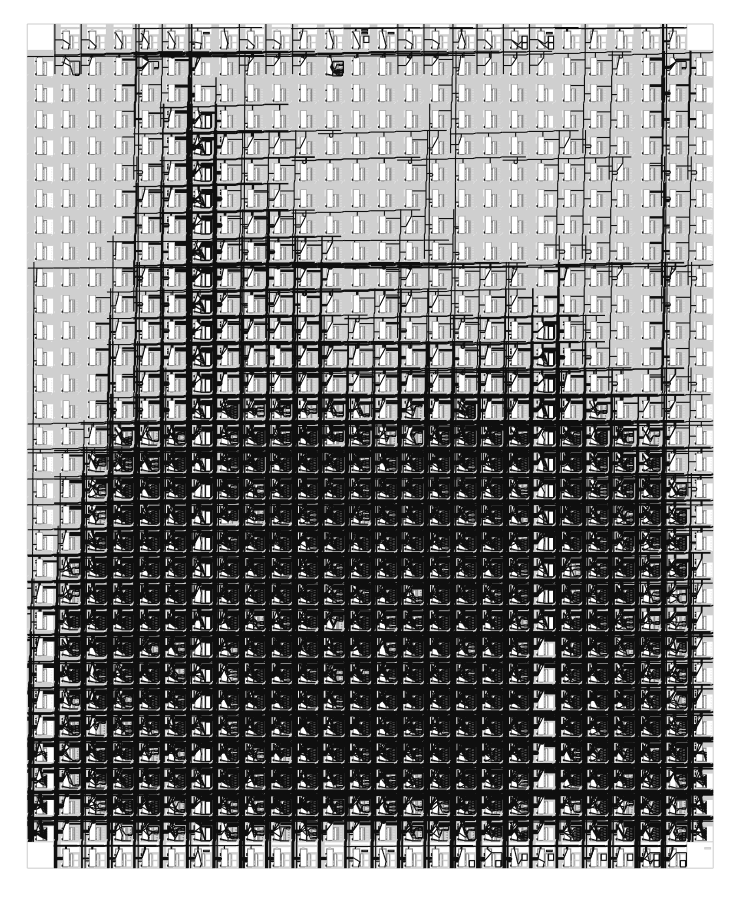
\includegraphics[width=.5\textwidth]{figures/fabric-full.png}};
		\draw[white, fill] (1,0) circle(3.5mm);
		\draw[white, line width=2mm]
			(130:3.1) ++(5,0) coordinate(top)
			(-130:3.1)++(5,0) coordinate(bottom)
			(130:.25)  ++(1,0) -- (top)
			(-130:.25) ++(1,0) -- (bottom);
		\begin{scope}[even odd rule]
			\draw[white, fill] (5,0) circle(3.2cm);
			\draw[black, ultra thick, fill=white] (5,0) circle(3.1cm);
			\clip (5,0) circle(3cm);
			\node (image) at (5,0) {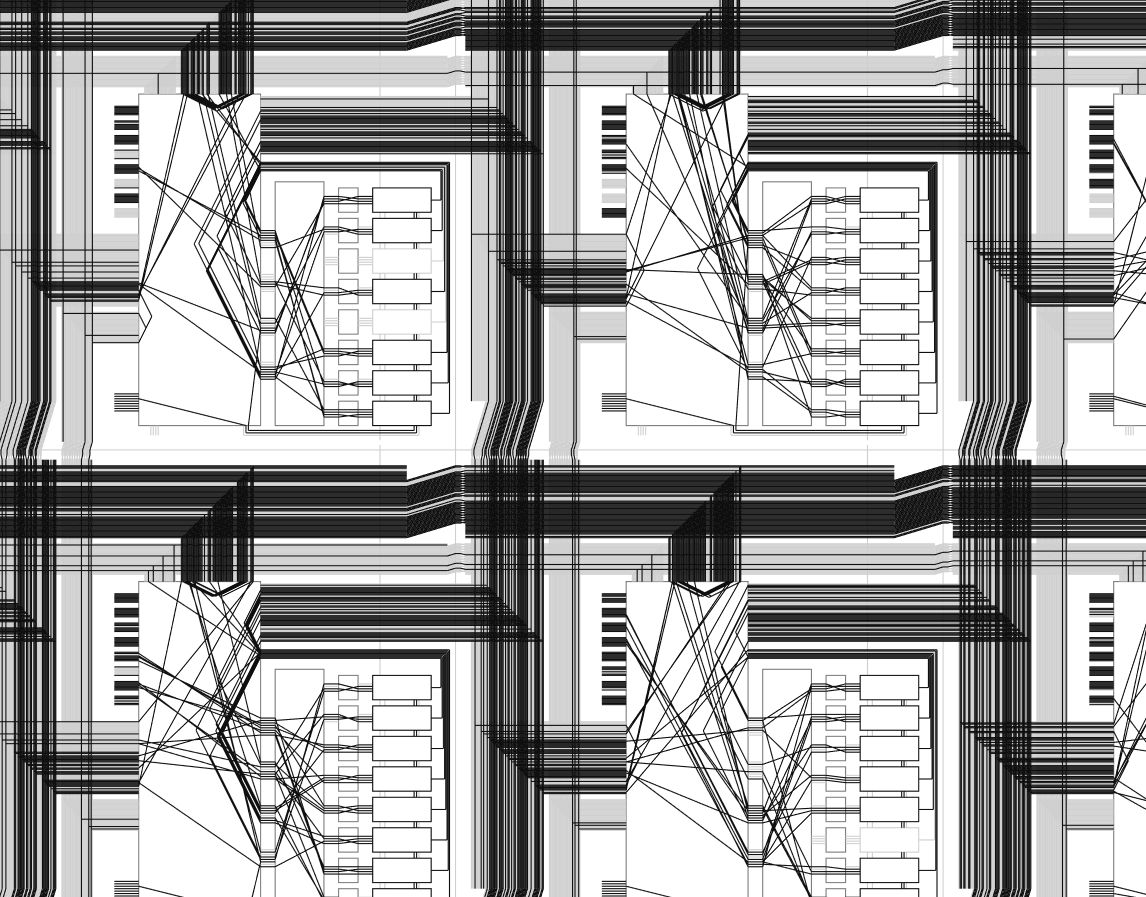
\includegraphics[height=6cm]{figures/fabric-zoom.png}};
		\end{scope}
		\draw[black, ultra thick]
			(130:3.1) ++(5,0) coordinate(top)
			(-130:3.1)++(5,0) coordinate(bottom)
			(130:.25)  ++(1,0) -- (top)
			(-130:.25) ++(1,0) -- (bottom);
		\draw[black, ultra thick, fill=white] (1,0) circle(2.5mm);
	\end{tikzpicture}
	\caption{Place and route output of my hardware design. The black wires represent the allocated interconnects. The zoomed portion shows the reconfigurable internals of several logic cells.}%
	\label{fig:pnr}
\end{figure}

HDL stands for ``hardware description language'' and it's the equivalent of ``code'' in software programming. Rather than code, a compiler, and an executable, the FPGA build toolchain has HDL, synthesis, place \& route, and the bitstream. I used the Verilog language to define the coprocessor, which is used to define state machines and combinational logic at the register-transfer level of abstraction. Synthesis is the process of turning this description into an abstract hardware definition. Place \& route is the process of placing circuit components onto elements of the FPGA fabric and routing connections between these components. Once the final FPGA configuration has been determined, it is serialized into a format that the FPGA chip can read to configure itself\cite{IceStorm}.

The FPGA configuration is volatile, so the bitstream must be sent to the chip each time the board turns on. The FPGA development board therefore includes a nonvolatile flash memory chip which stores the configuration bitstream and sends it to the FPGA when the board receives power\cite{iCEBreaker}.
